\section{Baseline 1}
\subsection{Pressupostos}

Os pressupostos usados para a \emph{Baseline 1} serão tudo aquilo que é usado como base para a criação da mesma. Dito isto, temos então três pilares essenciais sendo eles o âmbito, a equipa e a duração do projeto.

\addSubChapter{ambito}

\addSubChapter{equipa}

\addSubChapter{cronograma}

\subsection{Resultado}

Usando os pressupostos previamente detalhados, é alcaçada com sucesso, a \textit{baseline 1} e com a mesma concluida conseguimos ter as primeiras vistas sobre o projeto através das várias \textit{dashboards}, vistas de custos e vistas sobre os recursos facultadas pelo \textit{Microsoft Project}.

\begin{center}
    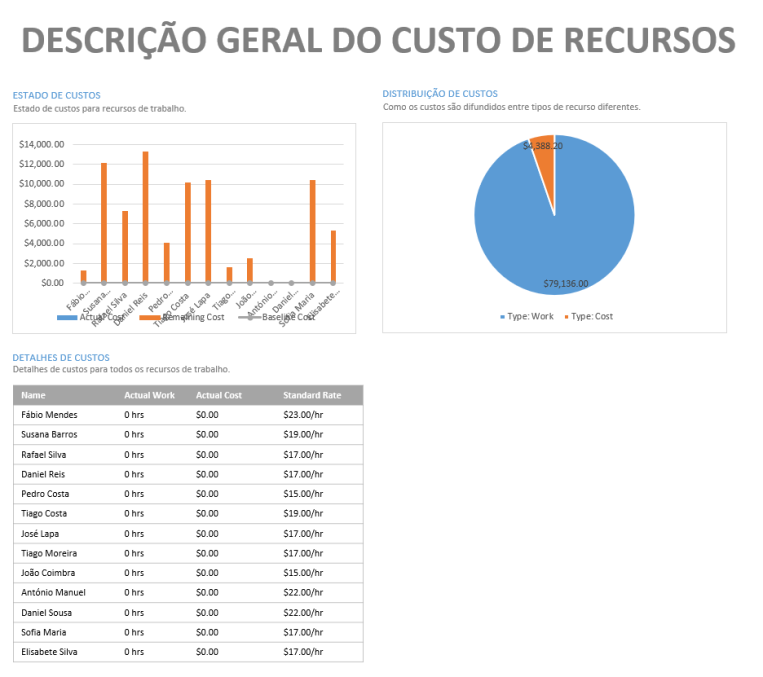
\includegraphics[width=0.7\textwidth]{media/baseline1Costs.PNG}
    \captionof{figure}{\textit{Baseline 1} - Descrição Geral do custo de Recursos}
\end{center}

\begin{center}
    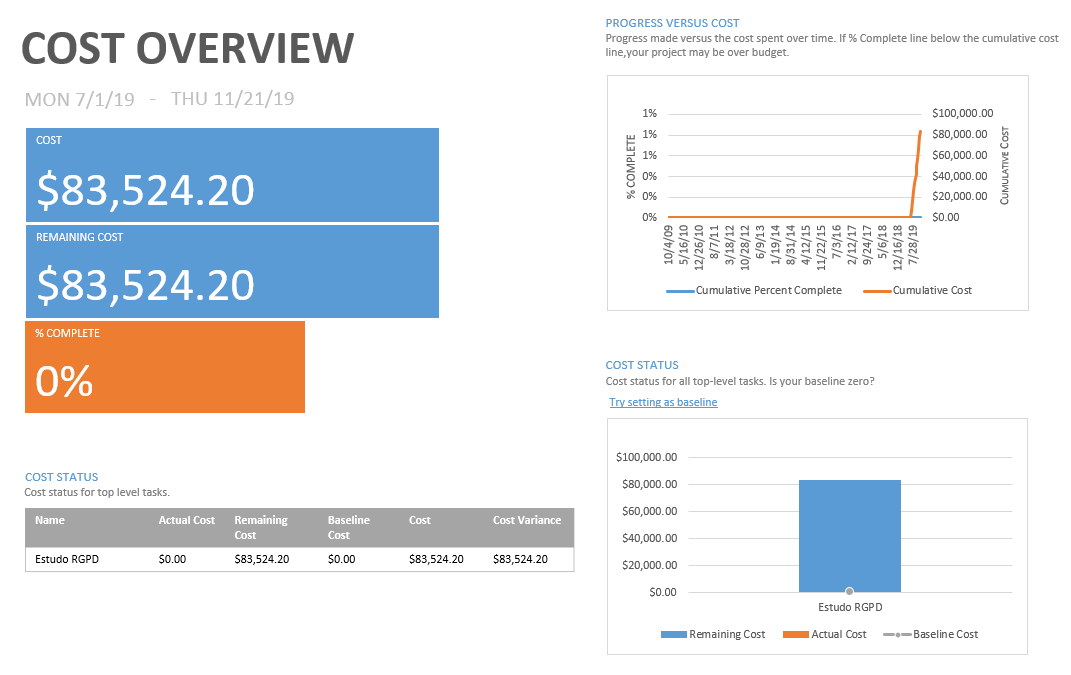
\includegraphics[width=0.7\textwidth]{media/baseline1CostOverview.PNG}
    \captionof{figure}{\textit{Baseline 1} - \textit{Cost Overview}}
\end{center}

Como nos encontramos na \textit{baseline 1}, obviamente que o projeto se encontra a 0\%, projeto esse que terá um custo de 83,524.20\$ e conseguimos através do gráfico perceber como esse custo está dividido sobre os recursos.